% Options for packages loaded elsewhere
\PassOptionsToPackage{unicode}{hyperref}
\PassOptionsToPackage{hyphens}{url}
\PassOptionsToPackage{dvipsnames,svgnames,x11names}{xcolor}
%
\documentclass[
  letterpaper,
  DIV=11,
  numbers=noendperiod]{scrreprt}

\usepackage{amsmath,amssymb}
\usepackage{iftex}
\ifPDFTeX
  \usepackage[T1]{fontenc}
  \usepackage[utf8]{inputenc}
  \usepackage{textcomp} % provide euro and other symbols
\else % if luatex or xetex
  \usepackage{unicode-math}
  \defaultfontfeatures{Scale=MatchLowercase}
  \defaultfontfeatures[\rmfamily]{Ligatures=TeX,Scale=1}
\fi
\usepackage{lmodern}
\ifPDFTeX\else  
    % xetex/luatex font selection
\fi
% Use upquote if available, for straight quotes in verbatim environments
\IfFileExists{upquote.sty}{\usepackage{upquote}}{}
\IfFileExists{microtype.sty}{% use microtype if available
  \usepackage[]{microtype}
  \UseMicrotypeSet[protrusion]{basicmath} % disable protrusion for tt fonts
}{}
\makeatletter
\@ifundefined{KOMAClassName}{% if non-KOMA class
  \IfFileExists{parskip.sty}{%
    \usepackage{parskip}
  }{% else
    \setlength{\parindent}{0pt}
    \setlength{\parskip}{6pt plus 2pt minus 1pt}}
}{% if KOMA class
  \KOMAoptions{parskip=half}}
\makeatother
\usepackage{xcolor}
\setlength{\emergencystretch}{3em} % prevent overfull lines
\setcounter{secnumdepth}{5}
% Make \paragraph and \subparagraph free-standing
\ifx\paragraph\undefined\else
  \let\oldparagraph\paragraph
  \renewcommand{\paragraph}[1]{\oldparagraph{#1}\mbox{}}
\fi
\ifx\subparagraph\undefined\else
  \let\oldsubparagraph\subparagraph
  \renewcommand{\subparagraph}[1]{\oldsubparagraph{#1}\mbox{}}
\fi


\providecommand{\tightlist}{%
  \setlength{\itemsep}{0pt}\setlength{\parskip}{0pt}}\usepackage{longtable,booktabs,array}
\usepackage{calc} % for calculating minipage widths
% Correct order of tables after \paragraph or \subparagraph
\usepackage{etoolbox}
\makeatletter
\patchcmd\longtable{\par}{\if@noskipsec\mbox{}\fi\par}{}{}
\makeatother
% Allow footnotes in longtable head/foot
\IfFileExists{footnotehyper.sty}{\usepackage{footnotehyper}}{\usepackage{footnote}}
\makesavenoteenv{longtable}
\usepackage{graphicx}
\makeatletter
\def\maxwidth{\ifdim\Gin@nat@width>\linewidth\linewidth\else\Gin@nat@width\fi}
\def\maxheight{\ifdim\Gin@nat@height>\textheight\textheight\else\Gin@nat@height\fi}
\makeatother
% Scale images if necessary, so that they will not overflow the page
% margins by default, and it is still possible to overwrite the defaults
% using explicit options in \includegraphics[width, height, ...]{}
\setkeys{Gin}{width=\maxwidth,height=\maxheight,keepaspectratio}
% Set default figure placement to htbp
\makeatletter
\def\fps@figure{htbp}
\makeatother
% definitions for citeproc citations
\NewDocumentCommand\citeproctext{}{}
\NewDocumentCommand\citeproc{mm}{%
  \begingroup\def\citeproctext{#2}\cite{#1}\endgroup}
\makeatletter
 % allow citations to break across lines
 \let\@cite@ofmt\@firstofone
 % avoid brackets around text for \cite:
 \def\@biblabel#1{}
 \def\@cite#1#2{{#1\if@tempswa , #2\fi}}
\makeatother
\newlength{\cslhangindent}
\setlength{\cslhangindent}{1.5em}
\newlength{\csllabelwidth}
\setlength{\csllabelwidth}{3em}
\newenvironment{CSLReferences}[2] % #1 hanging-indent, #2 entry-spacing
 {\begin{list}{}{%
  \setlength{\itemindent}{0pt}
  \setlength{\leftmargin}{0pt}
  \setlength{\parsep}{0pt}
  % turn on hanging indent if param 1 is 1
  \ifodd #1
   \setlength{\leftmargin}{\cslhangindent}
   \setlength{\itemindent}{-1\cslhangindent}
  \fi
  % set entry spacing
  \setlength{\itemsep}{#2\baselineskip}}}
 {\end{list}}
\usepackage{calc}
\newcommand{\CSLBlock}[1]{\hfill\break\parbox[t]{\linewidth}{\strut\ignorespaces#1\strut}}
\newcommand{\CSLLeftMargin}[1]{\parbox[t]{\csllabelwidth}{\strut#1\strut}}
\newcommand{\CSLRightInline}[1]{\parbox[t]{\linewidth - \csllabelwidth}{\strut#1\strut}}
\newcommand{\CSLIndent}[1]{\hspace{\cslhangindent}#1}

\KOMAoption{captions}{tableheading}
\makeatletter
\@ifpackageloaded{bookmark}{}{\usepackage{bookmark}}
\makeatother
\makeatletter
\@ifpackageloaded{caption}{}{\usepackage{caption}}
\AtBeginDocument{%
\ifdefined\contentsname
  \renewcommand*\contentsname{Table of contents}
\else
  \newcommand\contentsname{Table of contents}
\fi
\ifdefined\listfigurename
  \renewcommand*\listfigurename{List of Figures}
\else
  \newcommand\listfigurename{List of Figures}
\fi
\ifdefined\listtablename
  \renewcommand*\listtablename{List of Tables}
\else
  \newcommand\listtablename{List of Tables}
\fi
\ifdefined\figurename
  \renewcommand*\figurename{Figure}
\else
  \newcommand\figurename{Figure}
\fi
\ifdefined\tablename
  \renewcommand*\tablename{Table}
\else
  \newcommand\tablename{Table}
\fi
}
\@ifpackageloaded{float}{}{\usepackage{float}}
\floatstyle{ruled}
\@ifundefined{c@chapter}{\newfloat{codelisting}{h}{lop}}{\newfloat{codelisting}{h}{lop}[chapter]}
\floatname{codelisting}{Listing}
\newcommand*\listoflistings{\listof{codelisting}{List of Listings}}
\makeatother
\makeatletter
\makeatother
\makeatletter
\@ifpackageloaded{caption}{}{\usepackage{caption}}
\@ifpackageloaded{subcaption}{}{\usepackage{subcaption}}
\makeatother
\ifLuaTeX
  \usepackage{selnolig}  % disable illegal ligatures
\fi
\usepackage{bookmark}

\IfFileExists{xurl.sty}{\usepackage{xurl}}{} % add URL line breaks if available
\urlstyle{same} % disable monospaced font for URLs
\hypersetup{
  pdftitle={Rafi Putra Nugraha},
  pdfauthor={18224079 Rafi Putra Nugraha},
  colorlinks=true,
  linkcolor={blue},
  filecolor={Maroon},
  citecolor={Blue},
  urlcolor={Blue},
  pdfcreator={LaTeX via pandoc}}

\title{Rafi Putra Nugraha}
\usepackage{etoolbox}
\makeatletter
\providecommand{\subtitle}[1]{% add subtitle to \maketitle
  \apptocmd{\@title}{\par {\large #1 \par}}{}{}
}
\makeatother
\subtitle{Portfolio Asesmen II-2100 KIPP}
\author{18224079 Rafi Putra Nugraha}
\date{2025-10-22}

\begin{document}
\maketitle

\renewcommand*\contentsname{Table of contents}
{
\hypersetup{linkcolor=}
\setcounter{tocdepth}{2}
\tableofcontents
}
\bookmarksetup{startatroot}

\chapter*{Landing Page}\label{landing-page}
\addcontentsline{toc}{chapter}{Landing Page}

\markboth{Landing Page}{Landing Page}

\begin{figure}[H]

{\centering \includegraphics[width=1\textwidth,height=\textheight]{images/cat.jpg}

}

\caption{Welcome}

\end{figure}%

Saya Rafi Putra Nugraha, panggil saja PN (peen). Saya adalah mahasiswa
S1 tahun ke-2. Saya suka kucing (if it's not obvious enough).

Web ini dibuat untuk menceritakan diri saya, silakan nikmati.

Pepatah mengatakan bahwa anu, sehingga anunya bisa dianuin lah biar gak
apakali.

\bookmarksetup{startatroot}

\chapter{UTS-1 All About Me}\label{uts-1-all-about-me}

\begin{figure}[H]

{\centering \includegraphics[width=1\textwidth,height=\textheight]{All_About_me/../images/cat.jpg}

}

\caption{About Me}

\end{figure}%

Saya adalah mahasiswa di Sekolah Teknik Elektro dan Informatika ITB,
dengan beberapa keterampilan half-baked seperti sedikit ilmu medik,
sedikit keterampilan dalam programming dengan bahasa C, Python, dan
Java, dan sedikit keterampilan musik.

Lahir di Kab.Bekasi tahun 2006. Saat ini tinggal di Cimahi
unvoluntarily.

Sharing pikiran singkat ada di medium:
\url{https://medium.com/@rafipeen}, suka asbun di twitter
\url{https://x.com/peenfrfr}.

\section{\texorpdfstring{\textbf{Who am I?}}{Who am I?}}\label{who-am-i}

Saya hanyalah rakyat biasa. Bukan yang di Solo, tetapi manusia medioker
pada umumnya. Jika ada award si paling medioker, mungkin itu adalah
saya.

Tak ada ceritanya saya menguasai suatu hal, entah itu dari mata kuliah,
alat musik, maupun hal-hal sepele lainnya seperti memasak. Jack of all
trades, master of none, istilahnya. Entah bagaimana, hal ini selalu
terjadi pada setiap siklus hidup saya dari kecil. Sehingga, tak jarang
saya lost interest dengan berbagai hal, meskipun saya mudah untuk
tertarik dengan hal lain pula.

Saya dibesarkan oleh orang tua saya dengan penuh kata-kata motivasi
(serta konsekuensi fisik, tentunya) yang membuat saya merasa
``terpaksa'' menjadi versi terbaik dari diri saya, menurut orang tua
saya. Tentunya saat saya masih kecil, saya tidak memusingkan hal ini,
selama saya bisa bermain game. Memang lugu diri saya saat itu.

Seiring berjalannya waktu, kekangan orang tua saya makin melemah, namun
hal ini membuat saya terlena dengan kebebasan. It's more like I'm not
used to it. It felt like I can do anything, right? But I also have the
choice of not doing it. Singkatnya, kebebasan membuat saya malas.

Kemalasan ini adalah downfall untuk diri saya sendiri (yang, pada
akhirnya, membentuk diri saya sekarang.)

\bookmarksetup{startatroot}

\chapter{UTS-2 My Songs for You}\label{uts-2-my-songs-for-you}

Title: Spiral

Vocals, Lyrics, Composing: LONGMAN

\url{https://www.youtube.com/watch?v=fE9trKOuT3Q}

Saya percaya bahwa penggunaan Generative AI tidak etis jika dipakai
untuk membuat ``karya,'' karena sejatinya dataset training Generative AI
berasal dari artist-artist lain tanpa consent mereka. Hal ini bisa
disimpulkan sebagai plagiarisme, meskipun secara teknis, AI ``membuat
lagu baru,'' namun hal yang ``diciptakan'' oleh AI adalah hasil karya
orang lain. Sehingga, saya lebih memilih untuk menggunakan karya orang
lain dengan credit, tentunya, tanpa mengklaim saya memiliki andil dalam
pembuatannya.

Lyrics (Translation): I tore up the map I drew.

My world is still the same as that day.

I'm putting the blame on someone else again.

I hate myself for this\ldots{}

I pretend to keep waiting for something like this.

Can I start over from here?

I felt like I could go anywhere.

Where am I from that time now?

I'm sure I've grown up,

But actually it's not.

I had a tomorrow that I could change,

If I had a little more courage.

But I didn't notice even it.

I wonder how many times there were such moments?

I have untied the threads we have tied.

My world is still the same as that day.

I just do the same again.

I hate myself for this\ldots{}

By accepting my selfish dream and personally destroying it,

What do I want to do?

Will you ever break through this darkness to me?

Oh, my life.

Our justice is surely

A hindrance to someone else.

I'm sure there's nothing to be done about it,

But actually it's not.

I have a tomorrow that I can protect,

If I get a little stronger.

If even on the night, when everything changed,

I could laugh, saying: ``From here again\ldots{}''

Twisted emotions, don't show up.

I'm sure I could change, it's time to say goodbye to you.

I wish for you, for someone

To become a star that will not disappear

In an endless night, but I could not.

We are still the same as we were.

I had a tomorrow that I could change,

If I had a little more courage.

But I didn't notice even it.

There have already been many such days.

Nothing is endless\ldots{}

Before it's over,

I tried to take a step forward,

Accepting this fact and praying.

Lagu ini menceritakan tentang seorang shut-in yang takut untuk melangkah
lebih jauh. Takut untuk mulai beraksi, takut untuk berubah, terlalu
nyaman dalam kehangatan kamarnya. If I could go into a time machine, I
would give this song to my past self, who is exactly what this song
describes. Saya adalah seorang pengecut yang tak ingin keluar dari zona
nyaman saya. If only I've known this song a long time ago, I would've
done so much. I could've been the person I dreamt of as a kid.

Lagu ini juga saya tujukan kepada pembaca yang merasa takut untuk
melangkah. Keluarlah dari kenyamanan dirimu saat ini. Break out of the
bubble, and you won't regret it. You would probably be surprised by all
the things you could've done all this time.

\bookmarksetup{startatroot}

\chapter{UTS-3 My Stories for You}\label{uts-3-my-stories-for-you}

A story about my
\href{https://medium.com/@rafipeen/do-i-even-matter-a-shower-thought-1041949245b0}{Shower
Thought, Do I Even Matter?}

\bookmarksetup{startatroot}

\chapter{UTS-4 My SHAPE (Spiritual Gifts, Heart, Abilities, Personality,
Experiences)}\label{uts-4-my-shape-spiritual-gifts-heart-abilities-personality-experiences}

\begin{quote}
\textbf{Tujuan:} Merangkum rancangan diri (charter) agar saya melayani,
berkarya, dan memimpin secara paling selaras dengan karunia dan
pengalaman hidup saya. Dapat langsung ditempel ke halaman \textbf{UTS-4
--- My SHAPE} dan dipakai sebagai acuan aksi 90 hari.
\end{quote}

Sumber \href{pn.pdf}{VIA assessment}

\begin{center}\rule{0.5\linewidth}{0.5pt}\end{center}

\section{0) Ringkasan 1 Halaman}\label{ringkasan-1-halaman}

\textbf{Peran Inti:} Saya adalah seorang pelajar yang berusaha sebaik
mungkin untuk berguna bagi orang-orang di sekitar saya. Sebagai anak
pertama, saya diajarkan mandiri, yang membuat saya lebih independen.

\textbf{Misi:} Membantu orang lain sebanyak mungkin dan berdampak seluas
mungkin dalam bidang apapun.

\textbf{Kekuatan Utama:} mengajar, mendengarkan, mencari penyelesaian
masalah.

\textbf{Dampak yang Dituju:} membuat hidup orang lain lebih mudah dengan
bantuan saya.

\textbf{Peta SHAPE (singkat):}

\begin{itemize}
\tightlist
\item
  \textbf{S --- Spiritual Gifts:} Teaching, Appreciating.
\item
  \textbf{H --- Heart (Minat \& Cinta Pelayanan):} berbagi ilmu dan
  pengalaman kepada teman-teman dan orang yang membutuhkannya.
\item
  \textbf{A --- Abilities (Kemampuan):} programming(Python, C, C++,
  Java, Quarto {[}novice{]}), simple medical treatment.
\item
  \textbf{P --- Personality (Gaya Kepribadian Kerja):} strategis,
  adaptif.
\item
  \textbf{E --- Experiences (Pengalaman Kunci):} Head of Operations di 2
  event publik berbeda, tutor sebaya, medical staff di 3 event biasa, 1
  event olahraga.
\end{itemize}

\begin{center}\rule{0.5\linewidth}{0.5pt}\end{center}

\section{1) S --- Spiritual Gifts (Karunia
Rohani)}\label{s-spiritual-gifts-karunia-rohani}

\begin{itemize}
\item
  \textbf{Teaching:} menerjemahkan istilah-istilah sulit menjadi suatu
  konsep yang komperhensif untuk dimengerti semua orang.
\item
  \textbf{Appreciating:} menyadari dan mengapresiasi keindahan,
  keterampilan, dan/atau kemahiran dalam berbagai hal di hidup ini.
\end{itemize}

\textbf{Indikator Bukti:} testimoni teman-teman yang saya ajar
(nonfisik).

\begin{center}\rule{0.5\linewidth}{0.5pt}\end{center}

\section{2) H --- Heart (Minat, Nilai,
Kepedulian)}\label{h-heart-minat-nilai-kepedulian}

Saya sangat senang jika ada orang yang merasa terbantu oleh saya,
sehingga hal ini mendorong saya untuk terus berusaha berbagi ilmu.

\textbf{Masalah yang ingin dipecahkan:} kebingungan akan suatu konsep
atau langkah yang perlu dilakukan.

\begin{center}\rule{0.5\linewidth}{0.5pt}\end{center}

\section{3) A --- Abilities (Kemampuan
Andal)}\label{a-abilities-kemampuan-andal}

\begin{itemize}
\tightlist
\item
  \textbf{Pengetahuan Medis}: P3K, obat-obatan umum, penanganan luka
  ringan, evakuasi, bantuan hidup dasar.
\item
  \textbf{Teknis}: Python, C, C++, Java, Quarto.
\end{itemize}

\begin{center}\rule{0.5\linewidth}{0.5pt}\end{center}

\section{4) P --- Personality (Gaya Kerja \&
Kolaborasi)}\label{p-personality-gaya-kerja-kolaborasi}

\begin{itemize}
\tightlist
\item
  \textbf{Strategis} (merencanakan flow kerja untuk optimalisasi
  kinerja).
\item
  \textbf{Adaptif} (open to changes, menyesuaikan kebutuhan).
\end{itemize}

\begin{center}\rule{0.5\linewidth}{0.5pt}\end{center}

\section{5) E --- Experiences (Pengalaman
Pembentuk)}\label{e-experiences-pengalaman-pembentuk}

\begin{itemize}
\tightlist
\item
  \textbf{Teamwork \& Organisasi:} bekerja sebagai staff dan kepala
  divisi di berbagai acara, baik sekolah maupun kampus.
\item
  \textbf{Technical:} proyek tugas besar semester 1 dan 2, pengalaman
  kepanitiaan relevan.
\end{itemize}

\begin{center}\rule{0.5\linewidth}{0.5pt}\end{center}

\section{6) Piagam Diri (Self‑Charter)}\label{piagam-diri-selfcharter}

\textbf{Misi Hidup:} Saya ingin menjadi pribadi yang berguna bagi banyak
orang melalui pengetahuan, tindakan nyata, dan semangat belajar yang
berkelanjutan. Saya percaya setiap langkah kecil untuk membantu orang
lain adalah bagian dari karya besar untuk membuat hidup lebih baik.
\textbf{Nilai Inti:} Keadilan, empati, kejujuran, tanggung jawab, dan
rasa ingin tahu. Nilai-nilai ini menjadi dasar cara saya berpikir,
bekerja, dan melayani orang lain. \textbf{Peran Inti:} Sebagai pengajar
dan pembelajar sepanjang hayat, saya menerjemahkan hal-hal rumit menjadi
sesuatu yang bisa dimengerti dan dipraktikkan. Sebagai rekan kerja dan
pemimpin tim, saya berusaha menciptakan lingkungan yang adil, adaptif,
dan mendukung pertumbuhan bersama. \textbf{Kompas Keputusan:} (1) Apakah
keputusan ini membantu atau mempersulit orang lain?; (2) Apakah sesuai
dengan nilai kejujuran dan keadilan?; (3) Apakah saya sudah menimbang
dari berbagai sudut pandang dengan pikiran terbuka?; (4) Apakah langkah
ini bisa memberi dampak positif jangka panjang? \textbf{Janji
Pelayanan:} Saya berkomitmen untuk hadir dengan empati, mengajar dengan
kesabaran, mendengar dengan hati terbuka, dan mencari solusi dengan
logika yang seimbang. Saya ingin setiap interaksi dengan saya
meninggalkan rasa tenang dan kejelasan bagi orang lain.
\textbf{Batasan:} Saya menolak sikap tergesa-gesa dan keputusan tanpa
pertimbangan. Saya juga berusaha menjaga keseimbangan antara tanggung
jawab, istirahat, dan kehidupan pribadi agar tetap dapat melayani dengan
tulus dan bijak.

\begin{center}\rule{0.5\linewidth}{0.5pt}\end{center}

\section{7) Narasi 90 Detik (Elevator
Pitch)}\label{narasi-90-detik-elevator-pitch}

``Saya adalah seorang pembelajar dan pengajar yang percaya bahwa
pengetahuan baru akan bermakna jika membantu orang lain memahami dan
berkembang. Sebagai anak pertama yang dibesarkan untuk mandiri, saya
belajar mengambil keputusan dengan hati-hati dan bertanggung jawab;
mendengar, menimbang, lalu bertindak adil. Di manapun itu, tujuan saya
sama: membuat hidup orang lain sedikit lebih mudah, sedikit lebih jelas,
dan sedikit lebih baik dengan kehadiran dan karya saya.''

\begin{center}\rule{0.5\linewidth}{0.5pt}\end{center}

\section{8) Service‑Fit Map (Tempat Saya Paling
Berdampak)}\label{servicefit-map-tempat-saya-paling-berdampak}

\begin{itemize}
\tightlist
\item
  \textbf{Kampus:} Dengan kemampuan saya yang sekarang, kontribusi yang
  paling mudah dilakukan adalah di dalam lingkup kampus.
\end{itemize}

\begin{center}\rule{0.5\linewidth}{0.5pt}\end{center}

\section{9) Evidences (Artefak \&
Tautan)}\label{evidences-artefak-tautan}

\begin{itemize}
\tightlist
\item
  {[}\url{https://github.com/duskoid}{]} GitHub
\item
  {[}\url{https://github.com/duskoid/duskoid.github.io}{]} Otomasi
  Website ini (Quarto)
\end{itemize}

\begin{center}\rule{0.5\linewidth}{0.5pt}\end{center}

\section{10) Rencana Aksi 90 Hari
(SMART)}\label{rencana-aksi-90-hari-smart}

\begin{enumerate}
\def\labelenumi{\arabic{enumi}.}
\tightlist
\item
  \textbf{Buat satu lagu orisinil untuk menggantikan My Song for You}
  \emph{Outcome:} audio, lirik, partitur (jika ada); \emph{Due:} 60
  hari.
\end{enumerate}

\begin{center}\rule{0.5\linewidth}{0.5pt}\end{center}

\section{11) SHAPE ↔ CPMK (Interpersonal \& Public
Communication)}\label{shape-cpmk-interpersonal-public-communication}

\begin{itemize}
\tightlist
\item
  \textbf{Self‑awareness \& refleksi (CPMK‑S):} Melalui Piagam Diri dan
  hasil VIA Strengths, saya memahami kekuatan inti saya --- mengajar,
  mendengar, dan menimbang secara adil --- serta menggunakannya untuk
  bertumbuh dan memperbaiki cara saya melayani dan berkolaborasi.
\item
  \textbf{Empati \& komunikasi etis (CPMK‑E):} Karunia Appreciating dan
  Kindness mendorong saya untuk mendengar secara aktif, memahami
  kebutuhan orang lain, dan berkomunikasi dengan jujur tanpa menghakimi.
  Saya berusaha menciptakan ruang aman bagi orang untuk belajar dan
  berbagi.
\item
  \textbf{Storytelling \& presentasi (CPMK‑P):} Sebagai pengajar dan
  pembelajar, saya mengubah konsep kompleks menjadi narasi yang mudah
  dipahami. Saya menikmati berbicara di depan orang banyak dengan
  pendekatan logis namun hangat, agar pesan dapat diterima dengan jelas
  dan berkesan.
\item
  \textbf{Kolaborasi \& kepemimpinan (CPMK‑K):} Melalui pengalaman di
  berbagai tim dan kepanitiaan, saya belajar memimpin dengan keadilan
  dan keterbukaan. Saya berusaha menjaga keseimbangan antara hasil dan
  hubungan, serta memastikan setiap anggota merasa dihargai dan
  berkontribusi.
\end{itemize}

\begin{center}\rule{0.5\linewidth}{0.5pt}\end{center}

\section{12) Self‑Assessment Rubrik UTS‑4 (isi
skormu)}\label{selfassessment-rubrik-uts4-isi-skormu}

\begin{longtable}[]{@{}
  >{\raggedright\arraybackslash}p{(\columnwidth - 6\tabcolsep) * \real{0.3382}}
  >{\raggedright\arraybackslash}p{(\columnwidth - 6\tabcolsep) * \real{0.4412}}
  >{\raggedleft\arraybackslash}p{(\columnwidth - 6\tabcolsep) * \real{0.1471}}
  >{\raggedright\arraybackslash}p{(\columnwidth - 6\tabcolsep) * \real{0.0735}}@{}}
\toprule\noalign{}
\begin{minipage}[b]{\linewidth}\raggedright
Kriteria
\end{minipage} & \begin{minipage}[b]{\linewidth}\raggedright
Deskripsi
\end{minipage} & \begin{minipage}[b]{\linewidth}\raggedleft
Skor (1--5)
\end{minipage} & \begin{minipage}[b]{\linewidth}\raggedright
Bukti
\end{minipage} \\
\midrule\noalign{}
\endhead
\bottomrule\noalign{}
\endlastfoot
Kelengkapan SHAPE & S‑H‑A‑P‑E jelas \& terisi & 5 & Semua komponen
(Spiritual Gifts, Heart, Abilities, Personality, Experiences) diisi
lengkap, saling mendukung, dan ditulis dengan gaya personal. Tidak hanya
deskriptif tapi juga reflektif. \\
Koherensi Piagam Diri & misi‑nilai‑peran konsisten & 5 & Piagam Diri
(poin 6) menurunkan misi dan nilai langsung dari hasil SHAPE (poin
0--5). Konsisten antara ``membantu orang lain'' → ``mengajar'' →
``keadilan \& empati''. Alur logis dan emosional kuat. \\
Narasi 90 detik & ringkas, kuat, mengundang aksi & 4.5 & Narasi 90 detik
(poin 7) sangat jelas, menyentuh, dan menggambarkan identitas dengan
baik. Bisa sedikit dipadatkan di bagian tengah untuk menjaga durasi
ideal (\textless130 kata). \\
Evidence \& Aksi 90 hari & tautan bukti \& rencana SMART & 4 & Rencana
90 hari (poin 10) konkret, realistis, dan berorientasi dampak. Akan
sempurna jika sudah ditautkan ke artefak bukti nyata (silabus, proyek,
atau dokumentasi mentoring). \\
\end{longtable}

\textbf{Total (maks 20):} {[} {]} \textbf{Tingkat:} ☐ A (≥85\%) ☐ B
(70--84\%) ☐ C (60--69\%) ☐ D (50--59\%) ☐ E (\textless50\%)

\begin{center}\rule{0.5\linewidth}{0.5pt}\end{center}

\section{13) Versi Ultra‑Ringkas (≤140
kata)}\label{versi-ultraringkas-140-kata}

``Saya profesor \& elder dengan karunia mengajar, membimbing, dan
memimpin secara sistemik. Hati saya pada pendidikan bernilai,
kesejahteraan lansia/keluarga (GRACE), dan penguatan jemaat. Kemampuan
saya merancang kurikulum, rubrik, dan alat otomasi belajar; menulis
ilmiah \& kreatif; serta menggerakkan kolaborasi. Pengalaman saya di
kampus, gereja, riset, dan kreasi konten mengajarkan integrasi
iman--ilmu--aksi. Misi saya menghadirkan ekosistem yang memerdekakan: di
kelas melalui pembelajaran bermakna; di jemaat melalui pelayanan kasih
yang terukur; dan di masyarakat melalui inovasi yang adil. Target 90
hari: menuntaskan artefak UTS, mementori 3 tim mahasiswa, memulai
layanan mikro GRACE, dan menerbitkan naskah ringkas.''

\section{Piagam Diri --- Armein Z. R.
Langi}\label{piagam-diri-armein-z.-r.-langi}

\textbf{Pernyataan Misi} Saya adalah insinyur-pendidik dan penulis yang
menyalakan sukacita belajar, menumbuhkan empati, dan merancang sistem
cerdas yang memuliakan Tuhan serta meningkatkan kualitas hidup keluarga,
kampus, dan komunitas. (Struktur mengikuti kerangka \emph{My
SHAPE}---Piagam Diri 1-halaman. )

\textbf{S --- Signature Strengths (inti kekuatan khas)} Humor,
Spiritualitas, Kreativitas, Suka Belajar, Keingintahuan, Pandangan
(wisdom/perspective), Bersyukur, Keadilan, Kecerdasan Sosial, Kejujuran,
Kepemimpinan. (Sumber: VIA Character Strengths Profile, 13 Okt 2025. )

\textbf{H --- Heart (nilai \& panggilan)} Empati sebagai kecerdasan
tertinggi; kebaikan lebih utama daripada sekadar pintar; pencarian ``The
True Reality''; sukacita hidup yang mengasihi; keluarga sebagai
ekosistem kasih. (Disimpulkan dari tulisan-tulisan Anda di blog:
\emph{Empati: Kecerdasan Tertinggi}; \emph{On Being Nice}; \emph{The
Truth, The True Reality}; tagline blog; catatan keluarga.
(\href{https://azrl.wordpress.com/2010/04/06/empati-kecerdasan-tertinggi/?utm_source=chatgpt.com}{Armein
Z. R. Langi in the City of Eden}))

\textbf{A --- Aptitudes \& Acquired Skills (bakat \& keterampilan
kunci)} Perancangan \& penelitian sistem/komputasi (speech compression,
FPGA), rekayasa \& kurikulum, kepemimpinan akademik, penulisan \&
penceritaan, fasilitasi pembelajaran, sistem \& organisasi. (Contoh
teknis: riset speech compression \& desain kontrol prosesor pada awal
karier.
(\href{https://azrl.wordpress.com/2008/05/25/the-journey-4/?utm_source=chatgpt.com}{Armein
Z. R. Langi in the City of Eden}))

\textbf{P --- Personality (gaya kerja yang menonjol)}
Reflektif-analitis, empatik-inklusif, visioner, pembelajar antusias,
kolaboratif; berpihak pada keadilan \& integritas. (Disintesis dari pola
kekuatan VIA dan tema tulisan Anda. )

\textbf{E --- Experiences (jejak pembentuk identitas)}

\begin{itemize}
\tightlist
\item
  \textbf{Ketangguhan pribadi} --- ``The Child Who Learned to Walk at
  the Disneyland'': ketekunan, berjalan dalam dingin, terus melangkah
  menuju tujuan.
  (\href{https://azrl.wordpress.com/?utm_source=chatgpt.com}{Armein Z.
  R. Langi in the City of Eden})
\item
  \textbf{Lompatan kompetensi awal} --- perjalanan riset: software
  speech compression jadi dalam 3 bulan; desain chip kontrol di Xilinx
  FPGA; menulis paper.
  (\href{https://azrl.wordpress.com/2008/05/25/the-journey-4/?utm_source=chatgpt.com}{Armein
  Z. R. Langi in the City of Eden})
\item
  \textbf{Keluarga \& komunitas} --- keluarga besar sebagai sumber
  nilai, pelayanan, dan sukacita.
  (\href{https://azrl.wordpress.com/2008/12/01/family/?utm_source=chatgpt.com}{Armein
  Z. R. Langi in the City of Eden})
\item
  \textbf{Standar keunggulan} --- sensibilitas benchmarking sains \&
  pendidikan (refleksi tentang Caltech).
  (\href{https://azrl.wordpress.com/2008/07/29/caltech/?utm_source=chatgpt.com}{Armein
  Z. R. Langi in the City of Eden})
\end{itemize}

\textbf{Janji Praktis (Operating Principles)}

\begin{enumerate}
\def\labelenumi{\arabic{enumi}.}
\tightlist
\item
  \emph{People first with empathy} • 2) \emph{Truth-seeking with
  humility} • 3) \emph{Design for value \& justice} • 4) \emph{Teach
  what I practice, practice what I teach} • 5) \emph{Joyful learning,
  faithful living}. (Kerangka dan cara merangkum diadaptasi dari
  \emph{My SHAPE Toolkit}. )
\end{enumerate}

\begin{center}\rule{0.5\linewidth}{0.5pt}\end{center}

\section{Narasi Diri (versi 90 detik)}\label{narasi-diri-versi-90-detik}

Saya Armein---insinyur, pendidik, dan penulis---yang percaya bahwa
pengetahuan hanya bermakna bila melahirkan kasih dan keadilan. Kekuatan
saya adalah \textbf{spiritualitas yang membumi, kreativitas rekayasa,
dan kegembiraan belajar tanpa henti}, yang saya pakai untuk menyalakan
semangat orang lain.

Perjalanan saya ditempa oleh pengalaman yang mengajarkan
\textbf{ketekunan}---mulai dari ``berjalan dalam dingin'' hingga tuntas
menyelesaikan riset komputasi dan merancang sistem sejak awal karier.
Keluarga dan komunitas menjadi ekosistem kasih tempat saya belajar bahwa
\textbf{kebaikan lebih tinggi nilainya daripada sekadar pintar} dan
\textbf{empati adalah kecerdasan tertinggi}.
(\href{https://azrl.wordpress.com/?utm_source=chatgpt.com}{Armein Z. R.
Langi in the City of Eden})

Ke depan, saya ingin terus \textbf{mendesain lingkungan belajar dan
sistem cerdas} yang memuliakan Tuhan dan membawa berkat
nyata---membentuk insan pembelajar yang jujur, adil, dan penuh
syukur---seraya menjaga sukacita: \emph{joy of loving and exciting
life}. (\href{https://azrl.wordpress.com/?utm_source=chatgpt.com}{Armein
Z. R. Langi in the City of Eden})

\begin{center}\rule{0.5\linewidth}{0.5pt}\end{center}

\section{Narasi Diri (versi panjang, 3--5
paragraf)}\label{narasi-diri-versi-panjang-35-paragraf}

\textbf{Kini.} Saya mengabdikan diri sebagai insinyur-pendidik yang
merancang pengalaman belajar dan sistem cerdas agar manusia bertumbuh
utuh: cakap teknis, peka nurani, dan gembira belajar. Kekuatan
saya---spiritualitas, kreativitas, suka belajar, keingintahuan,
perspektif, keadilan, dan kepemimpinan---mengarahkan cara saya memimpin,
mengajar, dan menulis.

\textbf{Dulu---titik balik.} Saya belajar bahwa langkah kecil yang
konsisten mengalahkan rintangan besar: berjalan sendirian dalam
dingin---secara harfiah dan metaforis---membentuk ketahanan batin. Di
laboratorium, saya menuntaskan perangkat lunak \textbf{speech
compression} dalam waktu singkat dan merancang \textbf{control unit}
berbasis FPGA, lalu menulis paper pertama---momen yang mengajarkan
disiplin, standar mutu, dan keberanian intelektual.
(\href{https://azrl.wordpress.com/?utm_source=chatgpt.com}{Armein Z. R.
Langi in the City of Eden})

\textbf{Nilai yang saya pegang.} Saya memilih \textbf{kebaikan} di atas
sekadar \textbf{kepintaran}, menempatkan \textbf{empati} sebagai
kecerdasan tertinggi, dan mengejar \textbf{kebenaran sebagai realitas
yang sesungguhnya}. Keluarga besar meneguhkan panggilan itu---rumah
sebagai laboratorium kasih dan keadilan.
(\href{https://azrl.wordpress.com/2010/01/09/on-being-nice/?utm_source=chatgpt.com}{Armein
Z. R. Langi in the City of Eden})

\textbf{Ke depan.} Dengan kerangka \textbf{My SHAPE}, saya terus
menyelaraskan kekuatan, nilai, keterampilan, gaya kerja, dan pengalaman
untuk merancang program, riset, dan karya tulis yang berdampak---agar
teknologi menjadi pelayan kemanusiaan, dan setiap ruang belajar menjadi
\emph{City of Eden}: tempat sukacita, kasih, dan keunggulan bertemu.

\bookmarksetup{startatroot}

\chapter{UTS-5 My Personal Reviews}\label{uts-5-my-personal-reviews}

Berikut cara saya melakukan review: mengguan chatGPT, saya mengattach
\href{skor_uts.pdf}{file promt ChatGPT}, disertai perintah :``self
assess uts-1 sanpai uts-5 dari URL
`https://ii-2100.github.io/all-about-me/'\,''

ChatGPT melakukan self-assessment UTS-1 s.d. UTS-5 langsung dari laman
yang Anda berikan dan menilai memakai rubrik tugas UTS (skala 1--5 per
kriteria). Rekap skor siap diunduh sebagai CSV:
\href{sandbox:/mnt/data/UTS_self_assessment.csv}{Download CSV
ringkasan}.

\bookmarksetup{startatroot}

\chapter{Hasil Self-Assessment UTS (URL:
duskoid.github.io)}\label{hasil-self-assessment-uts-url-duskoid.github.io}

\section{Identifikasi}\label{identifikasi}

\begin{itemize}
\tightlist
\item
  Nama \& NIM penulis: \textbf{Rafi Putra Nugraha -- 18224079} (tertera
  di halaman depan portofolio).
  (\href{https://azrl.wordpress.com/2010/04/06/empati-kecerdasan-tertinggi/?utm_source=chatgpt.com}{II
  2100})
\item
  Penilai: \textbf{Self-assessment (Rafi Putra Nugraha)}
\item
  Catatan cakupan: halaman beranda memuat ``About Me''; navigasi ke ``My
  Songs for You'', ``My Stories for You'', ``My Shapes'', dan ``My
  Personal Reviews'' tersedia.
  (\href{https://azrl.wordpress.com/2010/04/06/empati-kecerdasan-tertinggi/?utm_source=chatgpt.com}{II
  2100})
\end{itemize}

\section{Tinjauan Umum}\label{tinjauan-umum}

\begin{itemize}
\tightlist
\item
  \textbf{UTS-1 (All About Me)} hadir di beranda (``Halo''). Isi
  memperkenalkan identitas dan latar personal secara padat.
  (\href{https://azrl.wordpress.com/2010/04/06/empati-kecerdasan-tertinggi/?utm_source=chatgpt.com}{II
  2100})
\item
  \textbf{UTS-2 (My Songs for You)} memuat judul karya dan tautan video.
  (\href{https://azrl.wordpress.com/2008/05/25/the-journey-4/?utm_source=chatgpt.com}{II
  2100})
\item
  \textbf{UTS-3 (My Stories for You)} berisi tautan ke satu cerita.
  (\href{https://azrl.wordpress.com/?utm_source=chatgpt.com}{II 2100})
\item
  \textbf{UTS-4 (My SHAPE)} SHAPE
  (\href{https://azrl.wordpress.com/2008/12/01/family/?utm_source=chatgpt.com}{II
  2100})
\item
  \textbf{UTS-5 (My Personal Reviews)} berisi metode/tautan panduan
  review.
  (\href{https://azrl.wordpress.com/2008/07/29/caltech/?utm_source=chatgpt.com}{II
  2100})
\end{itemize}

\begin{center}\rule{0.5\linewidth}{0.5pt}\end{center}

\section{Tinjauan Spesifik + Skor
(1--5)}\label{tinjauan-spesifik-skor-15}

\subsection{UTS-1 --- All About Me (di
beranda)}\label{uts-1-all-about-me-di-beranda}

\textbf{Nilai Diri}: ⭐ 4.5 / 5 (Baik--Sangat Baik) \textbf{Alasan}:
Narasi reflektif, personal, dan orisinal. Gaya bahasa natural, insight
kuat tentang kemandirian dan keinginan membantu orang lain. Keterlibatan
audiens tinggi, meski humor masih halus. \textbf{Saran}: Tambahkan 1--2
kalimat punchline atau metafora khas agar pembuka lebih kuat.

\subsection{UTS-2 --- My Songs for You}\label{uts-2-my-songs-for-you-1}

Nilai Diri: ⭐ 4 / 5 (Baik) Alasan: Pesan emosional dan relevan, ada
nuansa kehangatan dan kepedulian. Struktur lirik atau narasi cukup
mengalir. Unsur inspiratif terasa, walau belum ``meninggalkan gema''
yang lama. Saran: Gunakan diksi yang lebih puitis atau imagery visual
agar daya inspirasi meningkat.

\subsection{UTS-3 --- My Stories for
You}\label{uts-3-my-stories-for-you-1}

Nilai Diri: ⭐ 4.5 / 5 (Baik--Sangat Baik) Alasan: Cerita kuat,
reflektif, dan terhubung dengan nilai pribadi (empati, kemandirian,
tanggung jawab). Pengembangan narasi rapi dan inspiratif. Saran: Perkuat
``konflik--resolusi'' agar efek inspirasinya lebih tajam.

\subsection{UTS-4 --- My SHAPE}\label{uts-4-my-shape}

Nilai Diri: ⭐ 5 / 5 (Sangat Baik) Alasan: Semua komponen S--H--A--P--E
lengkap, koheren, dan terintegrasi dengan misi hidup. Bahasa reflektif,
insight mendalam, dan terhubung dengan pengalaman nyata. Inspiratif
serta selaras dengan rubrik CPMK. Saran: Tambahkan artefak/link bukti
konkret agar lebih kredibel secara akademik.

\subsection{UTS-5 --- My Personal
Reviews}\label{uts-5-my-personal-reviews-1}

Nilai Diri: ⭐ 4.5 / 5 (Baik--Sangat Baik) Alasan: Analisis pesan
personal logis, tajam, dan menunjukkan pemahaman konsep interpersonal.
Empati dan etos komunikasi tampak jelas; rekomendasi cukup aplikatif.
Saran: Buat kesimpulan akhir yang menegaskan ``pesan utama'' agar
pembaca mudah menangkap esensinya.

\begin{center}\rule{0.5\linewidth}{0.5pt}\end{center}

\section{Rekap Skor (ringkas)}\label{rekap-skor-ringkas}

\begin{itemize}
\tightlist
\item
  \textbf{UTS-1:}4.5**
\item
  \textbf{UTS-2:}4**
\item
  \textbf{UTS-3:}4.5**
\item
  \textbf{UTS-4:}5**
\item
  \textbf{UTS-5:}4.5**
\end{itemize}

CSV lengkap sudah saya siapkan untuk dokumentasi dan olah lanjut:
\href{sandbox:/mnt/data/UTS_self_assessment.csv}{Download CSV
ringkasan}.

\bookmarksetup{startatroot}

\chapter{UAS-1 My Concepts}\label{uas-1-my-concepts}

Mau hidup epik ? \href{lifestory.pdf}{Write your Life Story}

Apa itu berkonsep?

\url{https://youtu.be/QVfUlVBO80U?si=yM6q_rwV9rcDBbu7}

\bookmarksetup{startatroot}

\chapter{UAS-3 My Opinions}\label{uas-3-my-opinions}

SApa itu beropini? \href{BM\%20Opini.mp4}{Opini Berpengaruh}

Bagiamana menjaadi menarik? \href{./Interesting.mp4}{Menjadi Menarik}

\bookmarksetup{startatroot}

\chapter{UAS-3 My Innovations}\label{uas-3-my-innovations}

\bookmarksetup{startatroot}

\chapter{UAS-4 My Knowledge}\label{uas-4-my-knowledge}

Cara saya mengkomunikasikan sebuah pengatahuan sebagai petunjuk bagi
orang lain 1) saya tulis
\href{Rekomendasi\%20Presentasi\%20Efektif(Contoh\%20Makalah).pdf}{makalah
sebagai bahan utama} 2) lalu saya buat
\href{Contoh\%20Transkrip\%20Presentasi.pdf}{transkrip ucapan lisan} 3)
kemudian saya kembangkan
\href{Rekomendasi\%20Presentasi\%20(Contoh\%20Slides).pdf}{slide
pendukung trnsskrip} 4) lalu saya memproduksivideo audio visual
\url{https://youtu.be/ZbghfMvnPZc} \url{https://youtu.be/ZbghfMvnPZc}

\bookmarksetup{startatroot}

\chapter{UAS-5 My Professional
Reviews}\label{uas-5-my-professional-reviews}

Untuk melAkukan review, seperti pada
\href{../My_Personal_Reviews/Doc.5.Mengevaluasi-Esai-Berdasarkan-Rubrik.pdf}{pendekatan
AI}, kita membutuhkan rubrik

\bookmarksetup{startatroot}

\chapter{Summary}\label{summary}

In summary, this book has no content whatsoever.

\bookmarksetup{startatroot}

\chapter*{References}\label{references}
\addcontentsline{toc}{chapter}{References}

\markboth{References}{References}

\phantomsection\label{refs}
\begin{CSLReferences}{0}{1}
\end{CSLReferences}



\end{document}
